\documentclass[11pt]{article}
\usepackage{theme}
\usepackage{shortcuts}
\usepackage{minted}
\usepackage[citestyle=alphabetic,bibstyle=alphabetic]{biblatex}
\addbibresource{main.bib}
\usemintedstyle{emacs}


\newenvironment{pseudocode}{
    \VerbatimEnvironment
    \begin{minted}[mathescape,
        style=manny,
        linenos,
        numbersep=5pt,
        gobble=2,
        frame=lines,
        escapeinside=||,
        framesep=2mm,
        rulecolor=magenta]{python}%
}{
    \end{minted}%
}



% Document parameters
% Document title
\title{Mini-Project (ML for Time Series) - MVA 2023/2024}
\author{
Esteban Christiann \email{mailto:esteban.christiann@ens-paris-saclay.fr} \\ % student 1
Alexi Canesse \email{mailto:alexi.canesse@ens-lyon.fr} % student 2
}

\begin{document}
\maketitle

\section{Introduction and contributions}

The article we studied~\cite{DECHEVEIGNE2018} introduce methods to preprocess electroencephalography (EEG) and magnetoencephalography (MEG) recordings. This type of data is really sensible and prone to artefacts that theses methods try to remove. The authors decided to publish all of their algorithms together because they are similar and form together, a whole pipeline.\\

The most obvious artefact appears in MEG data: steps/jump. They appear because the measurement of magnetic flux involves a feedback loop which can, when the flux varies too quickly, lose lock to the signal which creates a jump of fixed amplitude. Those jumps are followed by another type of artefact: ringing which happens because of the antialiasing hardware filter. They proposed algorithms to remove both of these artefacts. They also introduced algorithms for outliers detection and inpainting (removal of outliers/interpolation of missing data) that are less specific to MEG and EEG data. They also have an algorithm for robust detrending (not sensible to outliers) and robust rereferencing. \\

\begin{figure}
    \centering
    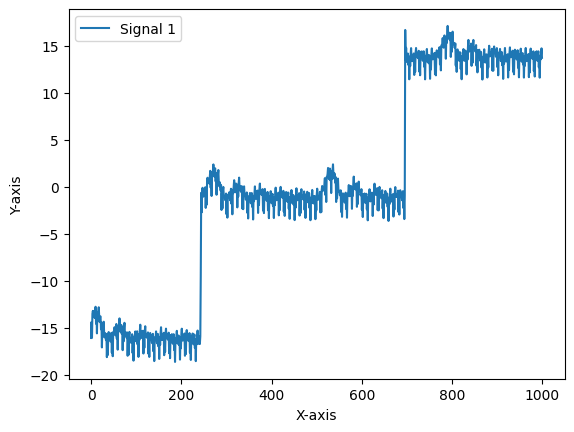
\includegraphics[width=.25\textwidth]{figures/steps_exemple}
    \hfill
    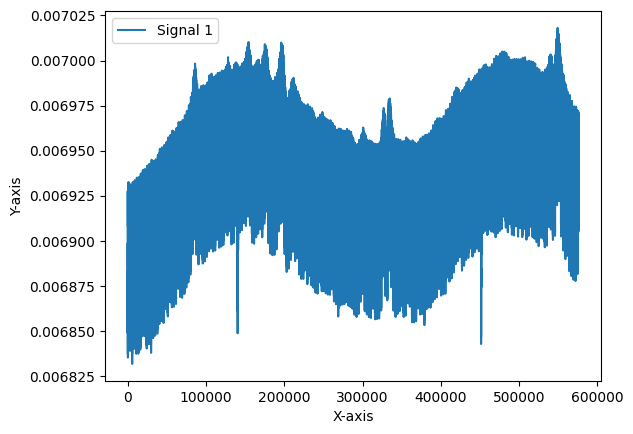
\includegraphics[width=.25\textwidth]{figures/trend_exemple}
    \hfill
    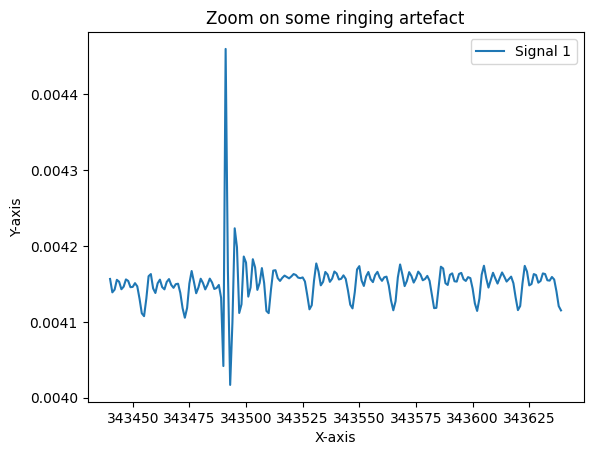
\includegraphics[width=.25\textwidth]{figures/ringing_exemple.png}
    \caption{Exemple of elements that the algorithms are here to remove. MEG steps on the left, trend on the middle and ringing on the right.}
\end{figure}

We implemented all of these algorithms in python. There is an existing implementation. However this implementation is in matlab so we did not use it. We also consider that \textbf{releasing code only in matlab is bad for reproducible science} and should not be considered as a proper release. We therefore did not used an existing implementation and took time to read this matlab code only to understand part of the algorithms that were not clear in the article (for instance notations such as \(d(t)/\text{STD}(d(t))\) is not only questionnable, it creates doubts about what the object really are and only looking at the implementation made it clear.).\\

Both students implemented some of the algorithms. Esteban implemented painting, outlier detection and ringing removal. Alexi implemented detrending, rereferencing, step removal. The data has been gathered and exploited as a combined efforts. The same goes for the experiments. This report has been written by both students with an equal repartition.\\

\section{Method}

The following section presents the algorithms proposed by the paper and gives pseudo-code for each algorithm.

\subsection{Robust detrending}

The main issue with usual detrending methods is that they are sensible to artefacts that are common in EEG and MEG data. They therefore present an algorithm that takes this into account. We fit a trend to the data and where the residuals are over a threshold, we flag the point as an outlier and do not take it into account to fit a the basis anymore. This is iterated a few times and gives great results. 

\begin{pseudocode}
detrending(signal):
    weights = [1, 1, |\(\dots\)|, 1] # weights for outlier detection (0 means outlier)
    iterrate |\(n_\text{iter}\)| times:
        projected_signal = fit_to_basis_using_weights(signal, weights)
        error_on_projection = abs(signal - projected_signal)
        for t in len(signal):
            if error_on_projection[t]/std(error_on_projection) > threshold:
                weights[t] = 0
            else:
                weights[t] = 1
    return signal - fitted_signal # detrended signal
\end{pseudocode}

\subsection{Inpainting}


\subsection{Outlier detection}


\subsection{Robust rereferencing}

Rereferencing is subtracting the average over all channels to the data. It is used because EEG measures are potentials therefore relative. When applying rereferencing, one corrupted channel can then affect every channels. To prevent this, the mean computed is computed only on values that are not outliers according to the outlier detection algorithm. Another solution is to use the output of the inpainting algorithm instead of the raw data.

\begin{pseudocode}
rereferencing(signal):
    weights = 1 - outlier_detection(signal) # 1 : valid data / 0 : outlier
    weighted_mean = mean_using_weights(signal, weights)
    return signal - weighted_mean
\end{pseudocode}

\subsection{Step removal}

The algorithm has two parts, first, it detects steps and then it removes them. In order to detect steps, the algorithm look at the empirical variance from the beginning and from the end and recursively look for the next step until it can't find any or the max depth is reached. We suspect that this part of the algorithm could be improved using change point detection methods we have seen in the fifth lab. However, we did not compared them because the proposed solution already worked more than well enough.

\begin{pseudocode}
# Recursively look for steps in the signal
step_detection(signal, depth)
    |\(\forall (t,T)\)| M[t][T] = mean(x[t:T+1])
    |\(\forall (t,T)\)| V[t][T] = |\(\sum_{i=t}^T (x_i - M_t^T)^2\)|
    
    t0 = argmin(V[1][t] + V[t][T], t) # most likely position to be a step
    if not(is_step(signal, t0)): # Check if t0 is indeed the position of a step
        return [] # no steps
    
    # Check for steps on both sides of t0
    steps_left = step_detection(signal[:t0], depth - 1)
    steps_right = t0 + step_detection(signal[t0:], depth - 1) # + t0 because signal si shifted

    return concatenate(steps_left, [t0], steps_right)

step_removal(signal, depth):
    steps = step_detection(signal, depth)

    for step in steps:
        signal[steps:] -= difference_mean_before_and_after_step(signal, step)

    return signal # Without steps

\end{pseudocode}

\subsection{Ringing removal}


\section{Data}
MEG and EEG data are medical recordings which make them a scare ressource. They should also be shared with great care. We used data from~\cite{Litvak2016}, the same data as the one used in the original article. The protocol used to record these MEG signals are described in ~\cite{oswal2016analysis}. The recordings we used are from ``phantom090715\_BrainampDBS\_20150709\_07.ds'' because this dataset is described as being the most realistic.\\

The data is sampled at 2,400Hz. Each recording is 4 minutes long and contains 303 channels. The data contains artefacts such trends, steps, ringing and outliers that are inherent to MEG recordings. Those have been presented in introduction. The the steps fixed amplitude of \(3.5.10^{-5}\) fT. The antialiasing filter is a low-pass filter which cuts off of 600 Hz resulting in a ringing time of 4.8ms.\\

We did not pre-process our data as the algorithms we use are the main steps of pre-processing. Only denoising is not presented in the methods here. We did not applied any denoising because denoising should be applied \textit{after} the application of the methods presented in the article. Indeed, artefacts could greatly impact denoising. Furthermore, MEG data is complicated and we do not understand the field enough to even know when we would remove actual data. The authors of the recording implemented two sensor-level denoising methods. They first used S3P-a technique based on eigenvalue decomposition of the complex cross-spectral density matrix (this technique is similar to SSA studied in the lectures); the second is pTSSS which defines subspaces using singular value decomposition. These successfully removed artefacts related to the stimulation and low level frequencies. However, this did not improved their ability to perform the task of their experiment.\\

We also manually generated some signals using the sum of a polynomial and white noise on top of which we added an artificial glitch. This was meant to be easy to use and interpret data.\\ 

\section{Results}
The Result section (indicative length : 1 to 2 pages) should display numerical simulations on real data. If you re-used some existing implementations, it is expected that this section develops new experiments that were not present in the original article. Results should be discussed not only based on quantitative scores but also on qualitative aspects. In particular (especially if your article focuses on black box methods), please provide some feedbacks whether the method was adapted to the data or not and whether the hypothesis behind the approach you used were validated or not.

TODO.

\newpage

\printbibliography[heading=bibintoc]


\end{document}
